\documentclass{article}

\usepackage[a4paper,width=160mm,top=25mm,bottom=20mm]{geometry}
\usepackage{fancyhdr}
\usepackage[utf8]{inputenc}
\usepackage[T1]{fontenc}
\usepackage[english]{babel}
\usepackage[usenames,dvipsnames,svgnames,table]{xcolor}
\usepackage{hyperref}
\usepackage{graphicx}
\usepackage{amssymb}
\usepackage{amsmath}
\usepackage{amsthm}
\usepackage{algorithm}
\usepackage{algorithmicx,algpseudocode}
\usepackage{draftwatermark}
% \usepackage[firstpage]{draftwatermark}

\DeclareMathOperator*{\argmax}{arg\,max}
\DeclareMathOperator*{\argmin}{arg\,min}

\newcommand\numberthis{\addtocounter{equation}{1}\tag{\theequation}}

\newtheorem{theorem}{Theorem}
\newtheorem{lemma}{Lemma}
\newtheorem{definition}{Definition}
\newtheorem{remark}{Remark}

\SetWatermarkText{\textbf{Draft}}
\SetWatermarkScale{5}
\SetWatermarkAngle{30}
\SetWatermarkFontSize{2cm}
% \SetWatermarkColor[rgb]{1,0,0}
\SetWatermarkColor[gray]{0.95}


\fancypagestyle{firstpage}{
    \fancyhead{}
    \renewcommand{\headrulewidth}{0.5pt}
}

\pagestyle{fancy}
\fancyhf{}
\renewcommand{\sectionmark}[1]{\markright{#1}}
% \fancyhead[L]{\rightmark} % L (left), R (right), C (center)
\fancyhead[R]{\rightmark}
\fancyfoot[R]{\thepage}

\allowdisplaybreaks


\title{A Brief Survey on Data Augmentation and Few-shot Learning}
\author{Fei Jie \\ \href{mailto:hfut\_jf@aliyun.com}{hfut\_jf@aliyun.com}}


\begin{document}

\maketitle
\thispagestyle{firstpage}

\begin{abstract}
It is common knowledge that the more data an ML algorithm has access to, the more effective it can be. Since the high cost of data labeling, often few supervised information is available. To reduce the required amount of data, various strategies and models were proposed to solve or alleviate this problem. This article tries to explore possible ways to improve models' performance in low-data regime, gain insights into development of this field, and relate to different methods. I first introduce some concepts and problems. Then, some methods about data augmentation and few-shot learning are introduced and categorized. When introdction of those two topics, two representative models are detailed to illustrate the general idea of mainstream methods. 
\end{abstract}

\section{Introduction}

Low-data regime will result in ML models' overfitting in training dataset, which furthermore degrades the ability of generalization to test dataset. Thus, some tricks have been proposed to alleviate this problem, such as regularization, dropout\cite{hinton2012improving}, batch normalization\cite{ioffe2015batch}, and layer normalization\cite{ba2016layer}. However in low data regimes, even these techniques fall short, since the the flexibility of the network is so high. We first introduce some terms or concepts related to our topics.

\paragraph{Data Augmentation} \cite{krizhevsky2012imagenet} is routinely used in classification problem. Often it is non-trivial to encode known \textbf{invariances} in a model. It can be easier to encode those invariances in the data instead by generating additional data items through transformations from existing data items. For example, the labels of handwritten characters should be invariant to small shifts in location, small rotations or shears, changes in intensity, changes in stroke thickness, changes in size etc. Almost all cases of data augmentation are from a prior known invariance. Traditional data augmentation operations include: \textit{random translations, rotations, flips, addition of Gaussian noise,} etc. Note that aforementioned transformations \textbf{do not affect the class}.

\paragraph{Few-shot Learning} is tasks that study the ability to learn from few examples \cite{garcia2017few}. When the classes covered by training instances and the classes we aim to classify are disjoint, this paradigm are called \textbf{zero-shot learning} \cite{wang2019survey}. If we only observe a single example of each possible before making a prediction about a test instance, we call it \textbf{one-shot learning} \cite{koch2015siamese}, which was firstly proposed in \cite{fei2006one}. Here, we give a formal problem setup on several different learning settings (few-shot learning, semi-supervised learning and active learning) from the perspective of image classification \cite{garcia2017few}. 

We consider input-output pairs $(\mathcal{T}_i,Y_i)_i$ drawn iid from a distribution $P$ of partially-labeled image collections 
\[
\mathcal{T}=\left\{ \{(x_1,l_1),\dots,(x_s,l_s)\}, \{\tilde{x}_1,\dots,\tilde{x}_r \}, \{\bar{x}_1,\dots,\bar{x}_t \},  x_i,\tilde{x}_j,\bar{x}_j\sim\mathcal{P}_l(\mathbb{R}^N)\right\},
\]
and $Y=(y_1,\dots,y_t)\in\{1,K\}^t$, for arbitrary values of $s,r,t$ and $K$, where $s$ is the number of labeled samples, $r$ is the number of unlabeled samples (r > 0 for the semi-supervised and active learning scenarios) and $t$ is the number of samples to classify. $K$ is the number of classes. $\mathcal{P}_l(\mathbb{R}^N)$ denotes a class-specific image distribution over $\mathbb{R}^N$. In our context, the targets $Y_i$ are associated with images categories of designated images $\hat{x}_1,\dots,\hat{x}_t\in \mathcal{T}_i$ with no observed label. Given a training set $\left\{(\mathcal{T}_i,Y_i)_i \right\}_{i\leq L}$, we consider the standard supervised learning objective
\[
\min_{\Theta}\frac{1}{L}\sum_{i\leq L}\ell(\Phi(\mathcal{T}_i;\Theta),Y_i)+\mathcal{R}(\Theta),
\]
using the model $\Phi(\mathcal{T};\Theta)=p(Y|\mathcal{T})$ and $\mathcal{R}$ is a standard regularization objective.

\paragraph{Few-shot Learning} When $r=0,t=1$ and $s=qK$, there is a single image in the collection with unknown label. If moreover each label appears exactly $q$ times, this setting is referred as the \textbf{$q$-shot, $K$-way learning}. An example of datasets setting in few-shot learning tasks can be found in figure \ref{fig:fewshot}.

\begin{figure}
\centering
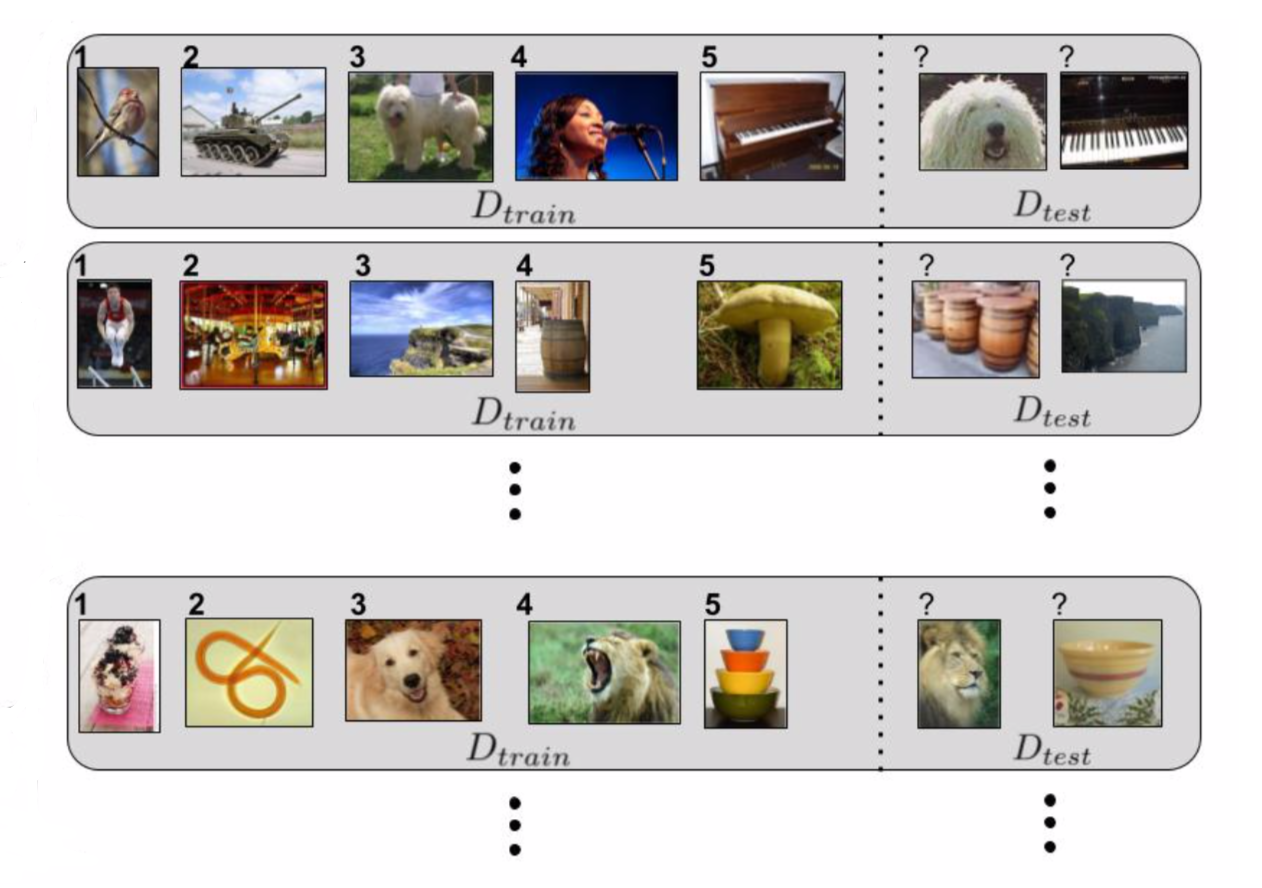
\includegraphics[width=10cm]{figures/fewshot}
\caption{Few-shot learning datasets setting. In few-shot leanring process, each training instance is a task (sometime we call it \textit{episode} \cite{vinyals2016matching}). Each task is separated $D_{\text{train}}$, $D_{\text{validation}}$ (ignored in this figure), $D_{\text{test}}$. In the training procedure of few-shot learning, a model takes one of $D_{\text{train}}$ datasets as input and produces a clssifier that achieves high average performance on its corresponding test set $D_{\text{test}}$. Using $D_{\text{validation}}$ we can perform hyper-parameter selection of the model and evaluate its generalization performance on $D_{\text{test}}$.}\label{fig:fewshot}
\end{figure}

\paragraph{Semi-supervised Learning} When $r>0$ and $t=1$, the input collection contains auxiliary images $\tilde{x}_1,\dots,\tilde{x}_r$ that model can use to improve the prediction accuracy, by leveraging the fact that these samples are drawn from common distributions as those determining the outputs.

\paragraph{Active Learning} In the active learning setting, the learner has the ability to request labels from the sub-collection $\{\tilde{x}_1,\dot,\tilde{x}_r \}$.


Some other terms related to this articles are Generative Adversarial Networks (GANs) \cite{goodfellow2014generative}, Transfer Learning, Meta Learning. I will introduce them when they are to be used.

% \paragraph{Generative Adversarial Networks} (GAN) \cite{goodfellow2014generative}, and specifically Deep Convolutional GANs (DCGAN)  use of the ability to discriminate between true and generated examples as an objective. GAN approaches can learn complex joint densities. Recent improvements in the optimization process have reduced some of the failure modes of the GAN learning process.


Except aforementioned tricks to overcome the lack of data and achieve few-shot learning, two intuitive solutions for this problems are \textbf{data augmentation} and \textbf{meta learning} \cite{sun2018meta}. Data augmentation is a intuitive strategy to increase the amount of available data and thus also useful for few-shot learning. In contrast to data-augmentation methods, meta-learning is a task-level learning method \cite{thrun2012learning}. {\color{red}{Meta-learning aims to accumulate experience from learning multiple tasks \cite{munkhdalai2017meta,ravi2016optimization,finn2017model}, while base-learning focuses on modeling the data distribution of a single task}}.

\section{Data Augmentation}

Data augmentation is one way we can reduce overfitting on models, where we increase the amount of training data using information \textbf{only in our training data}. Based on difference between deployment of data augmentation, it can be categorized into three classes:

\paragraph{Traditional Transformations} A very generic and accepted current practice for augmenting image data is to perform geometric and color augmentations, such as reflecting the image, cropping and translating the image, and changing the color palette of the image \cite{krizhevsky2012imagenet}. All of the transformation are affine transformation of the original image that take the form:
\[
y=Wx+b
\]

\paragraph{Generative Adversarial Networks} GANs \cite{goodfellow2014generative} has been a powerful technique to perform unsupervised generation of new images for training. They have also proven extremely effective in many data generation tasks. By using a min-max strategy, one neural net successively generates better counterfeit samples from the original data distribution in order to fool the other net. The other net is then trained to better distinguish the counterfeits. GANs have been used for style transfer such as transferring images in one setting to another setting (CycleGAN \cite{zhu2017unpaired}). These generated images could be used to train a car to drive in night or in the rain using only data collected on sunny days for instance. Furthermore, GANs have been effective even with relatively small sets of data \cite{gurumurthy2017deligan} by performing transfer learning techniques. We can use GANs or its variations to generate extra data. Note that in this setting the data augmentation model is independent of the classifiers \cite{perez2017effectiveness,antoniou2017data}, i.e., augmented data is generated before training the classifier.

A variation of GAN for data augmentation model DAGAN can be illustrated as figure \ref{fig:dagan} \cite{antoniou2017data}.

\begin{figure}[h]
\label{fig:dagan}
\centering
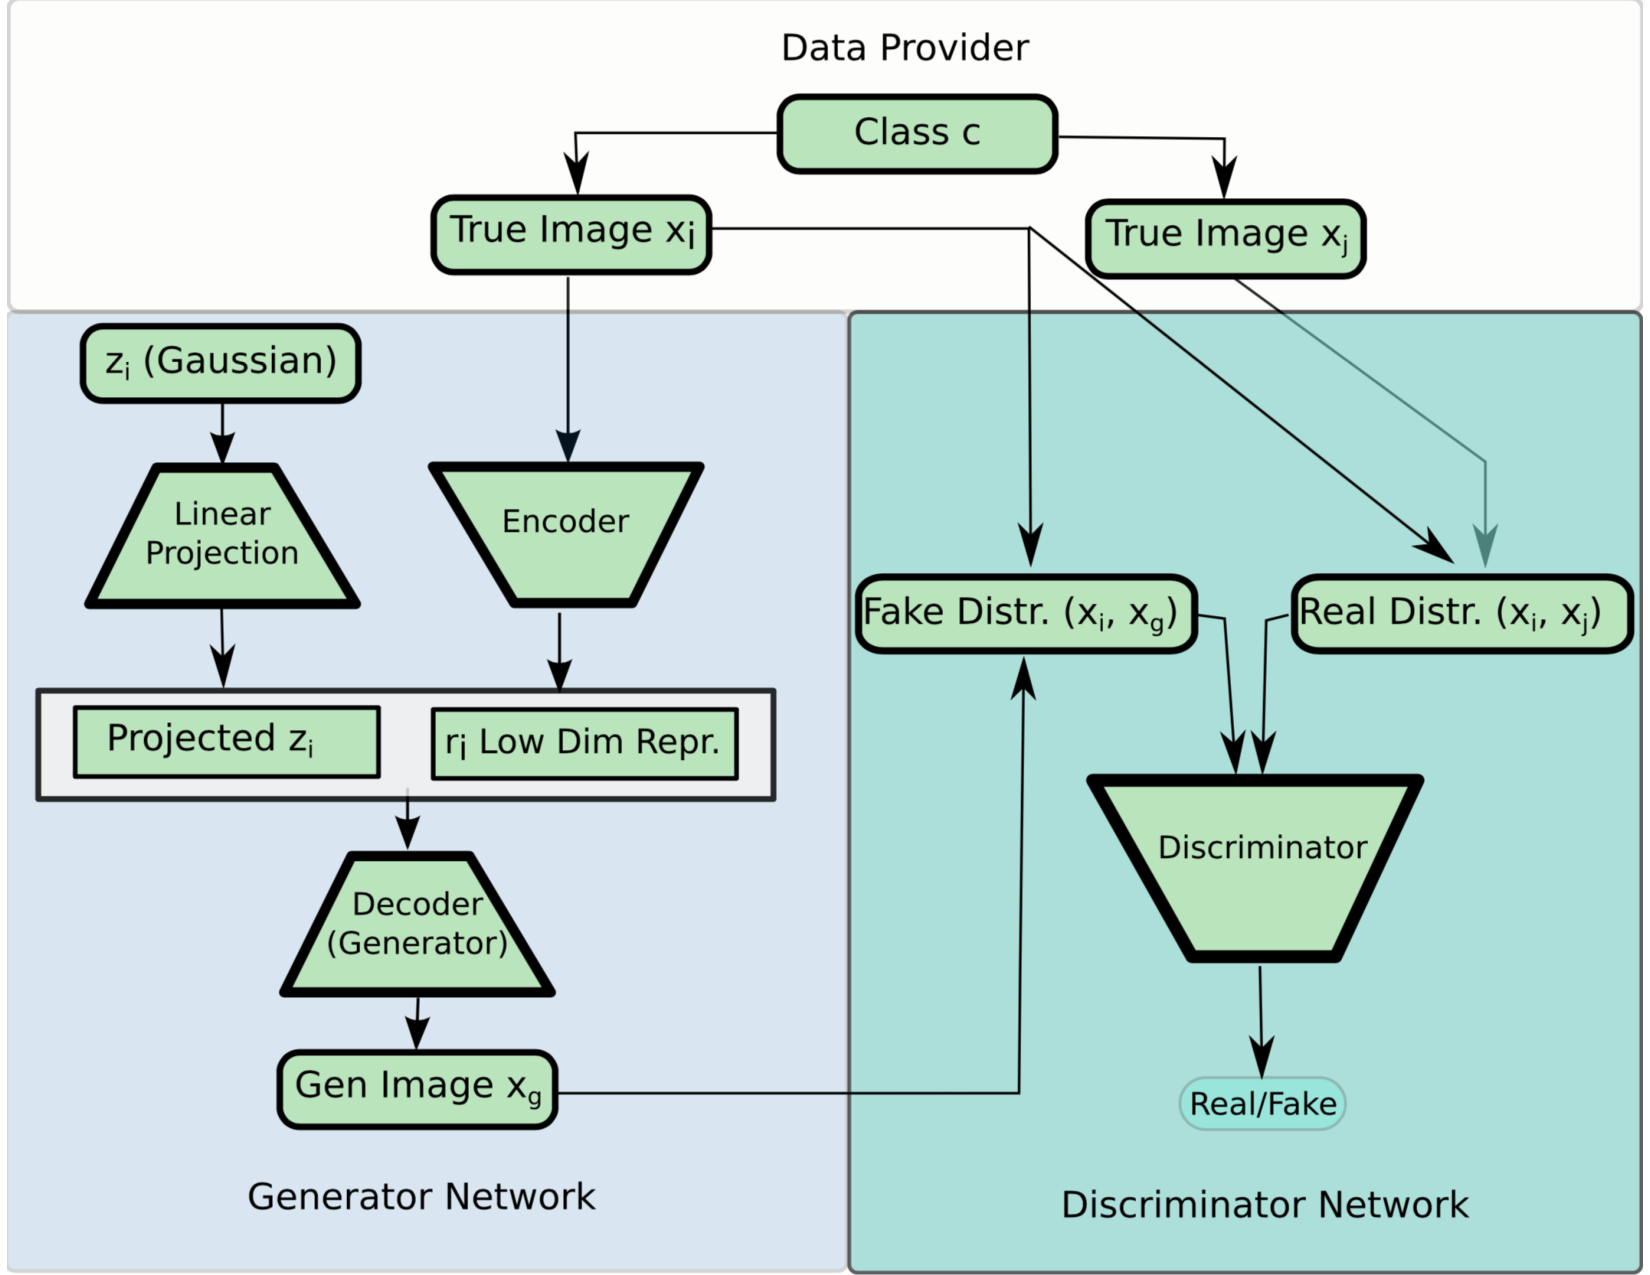
\includegraphics[width=8cm]{figures/dagan}
\caption{DAGAN Architecture. Left: the generator network is composed of an encoder taking an input image (from class c), projecting it down to a lower dimensional manifold (bottleneck). A random vector ($z_i$) is transformed and concatenated with the bottleneck vector; these are both passed to the decoder network which generates an augmentation image. Right: the adversarial discriminator network is trained to discriminate between the samples from the real distribution (other real images from the same class) and the fake distribution (images generative from the generator network). Adversarial training leads the network to generate new images from an old one that appear to be within the same class (whatever that class is), but look different enough to be a different sample.}
\end{figure}

DAGAN's generator differs from the standard GANs'. The generative model learnt by a Generative Adversarial Network (GAN) takes the form
\begin{gather*}
{\bf z}=\tilde{N}({\bf 0},{\bf I})\\
{\bf v}=f({\bf z})
\end{gather*}
where $f$ is implemented via a neural network. Here, ${\bf v}$ are the vectors being generated (that, in distribution, should match the data $D$), and ${\bf z}$ are the latent Gaussian variables that provide the
variation in what is generated. The generator of DAGAN model takes the form
\begin{gather*}
{\bf r}=g({\bf x})\\
{\bf z}=\tilde{N}({\bf 0},{\bf I})\\
{\bf v}=f({\bf z},{\bf r})
\end{gather*}
where the neural network $f$ now takes the representation ${\bf r}$ and the random ${\bf z}$ as inputs. Now given any new ${\bf x}^*$ we can
\begin{itemize}
\item Obtain a generative meaningful representation of the data point ${\bf r}^*=g({\bf x})$, that encapsulates the information needed to generate other related data.
\item Generate extra augmentation data ${\bf v}_1^*,{\bf v}_2^*,\dots$ that supplements the original ${\bf x}^*$, which can be used in a classifer. This can be done by sampling ${\bf z}$ from the standard Gaussian distribution and then using the generative network to generate an augmentation example.
\end{itemize}

\paragraph{Learning the Augmentation} This approach attempts to learn augmentation through a pre-pended neural net. At training time, the neural net takes data from the training set and outputs fake (augmented) data. Then the augmented data is fed into the classifier(e.g. a neural network) along with the original training data. The training loss is then backpropagated to train the augmenting layers of the networks as well as the classification layers of the network. In test time, instances from the validation or test set is ran through only the classification network. The motivation is to identify the best augmentations for a given dataset \cite{perez2017effectiveness}. Note that the training phase of learning the augmentation is similar with DVN \cite{gygli2017deep}, which both achieve {\color{red}{training and data augmentation simultaneously}}.
\begin{figure}[h]
\label{fig:cmb}
\centering
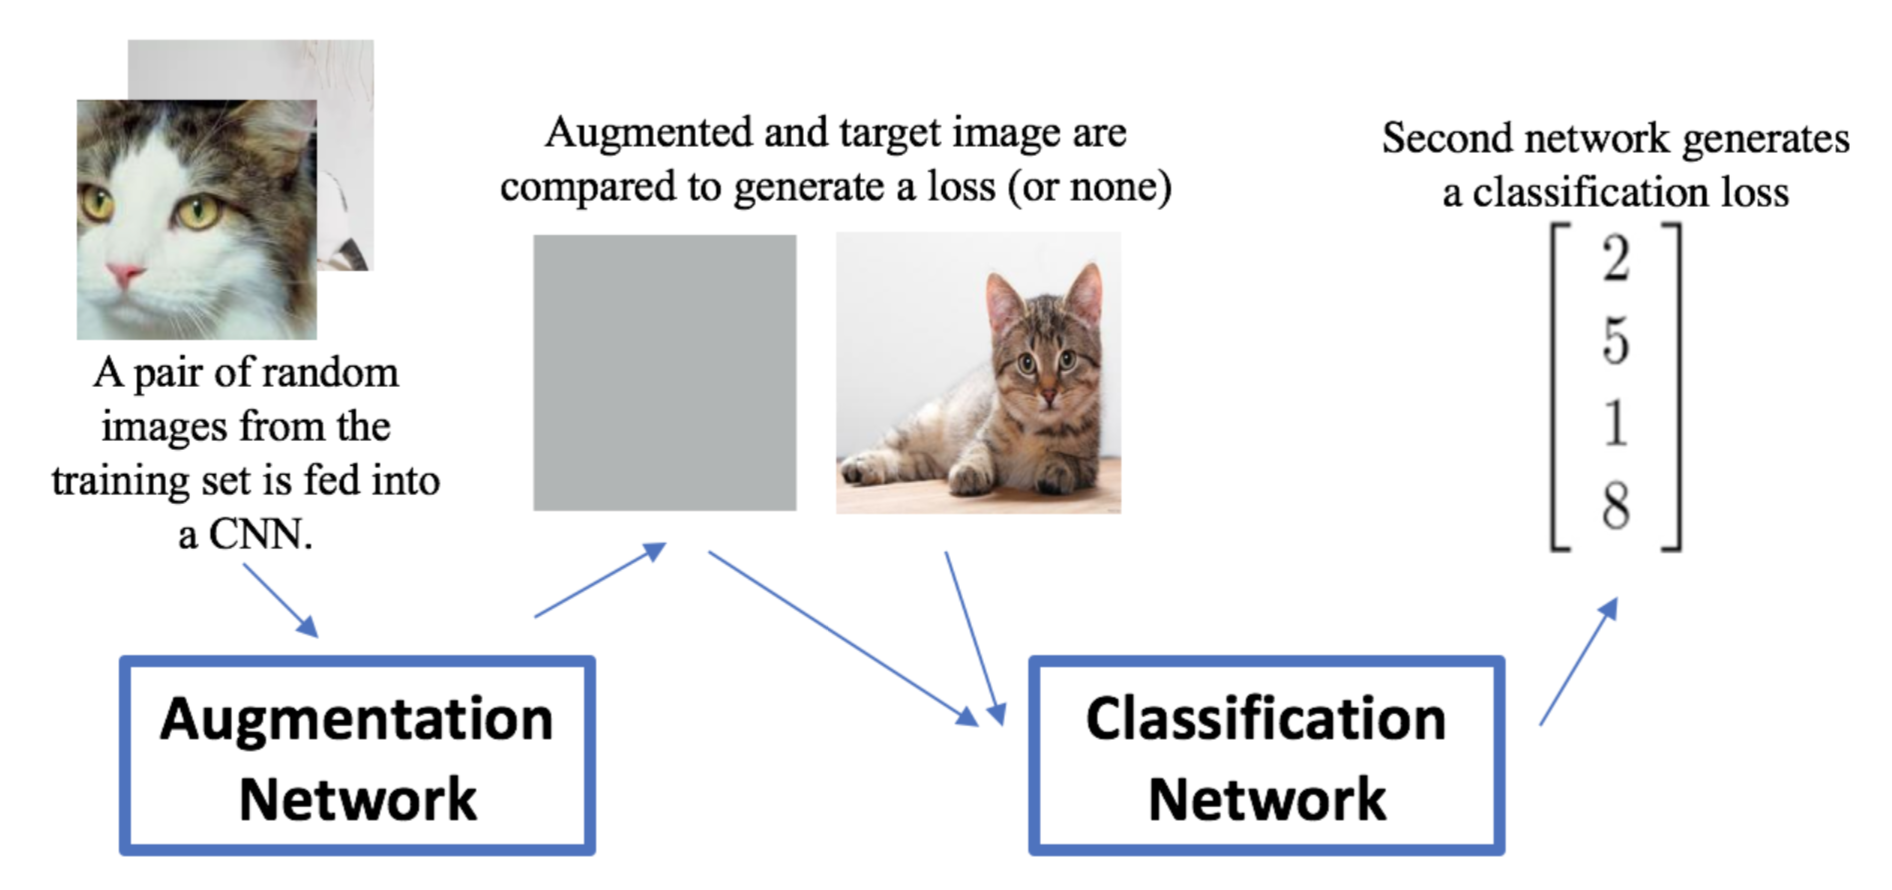
\includegraphics[width=10cm]{figures/learningaug}
\caption{Architecture of Learning the Augmentation model.}
\end{figure}

In the above model, except classification loss $_{\text{c}}$, we also include an augmentation loss $L_{\text{a}}$. Two augmentation losses can be considered. One is the content loss, which is the mean squared error between the augmentated imgae A and the target image $T$ and defined as
\[
L_{\text{a}}^{\text{content}}=\frac{1}{D^2}\sum_{i,j}(A_{i,j}-T_{i,j})
\]
where $D$ is the length of images A and $T$.

Another augmentation loss is the style loss, which is a content loss on the gram matrix of the augmentated image A and target image T. The gram matrix of feature map $F$ is defined below
\[
G_{i,j}=\sum_k F_{i,k}F_{j,k}
\]
Then the loss is defined below,
\[
L_{\text{a}}^{\text{style}}=\frac{1}{C^2}\sum_{i,j}(G_{i,j}^A-G_{i,j}^T)
\]
where $C$ is the number of channels.

Finally, the final loss is weighted sum of the two losses
\[
\alpha L_c+\beta L_a
\]

\section{Few-Shot Learning}

Another solution for low data regimes is few-shot learning. We can divide methods in this paradigm into several categories. 1) Metric/distance learning methods \cite{snell2017prototypical,sung2018learning,vinyals2016matching,koch2015siamese,mehrotra2017generative} learn a similarity space in which learning is particularly efficient for few-shot examples. 2) Meta learning \cite{munkhdalai2017meta,santoro2016meta,ravi2016optimization,finn2017model} learn to store “experience” when learning seen tasks and then generalize that to unseen tasks.

\subsection{Metric learning}

\cite{koch2015siamese} presented a deep learning model based on computing the pair-wise distance between samples using Siamese Networks, then, this learned distance can be used to solve one-shot problem by k-nearest neighbors classification. \cite{vinyals2016matching} presented an end-to-end trainable k-nearest neighbors using the cosine distance, they also introduce a contextual mechanism using an attention LSTM model \cite{hochreiter1997long} that takes into account all the samples of the subset $\mathcal{T}$ when computing the pair-wise distance between samples. \cite{snell2017prototypical} extended the work from \cite{vinyals2016matching}, by using euclidean distance instead of cosine which provided significant improvements, they also build a prototype representation of each class for the few-shot learning scenario. \cite{mehrotra2017generative} trained a deep residual network together with a generative model to approximate the pair-wise distance between samples.

\subsection*{Prototypical Networks}

I will use Prototypical Networks \cite{snell2017prototypical} as a instance to illustrate the idea of metric learning. The Prototypical Networks is based on the idea that {\color{red}{\textit{there exists an embedding in which points cluster around a single prototype representation for each class}}}. To do this, we learn a non-linear mapping of the input into an embedding space using a neural network and take a class's prototype to be the mean of its support set in the embedding space. 

Given a small support set of $N$ labeled examples $S=\{(x_1,y_1),\dots,(x_N,y_N)\}$ where each $x_i\in\mathbb{R}^D$ is the $D$-dimensional feature vector of an example and $y_i\in\{1,\dots,K \}$ is the corresponding label. $S_k$ denotes the set of examples labeled with class $k$. An illustration of the few-shot learning for Prototypical Networks is shown in figure \ref{fig:proto}.

\begin{figure}[h]
\centering
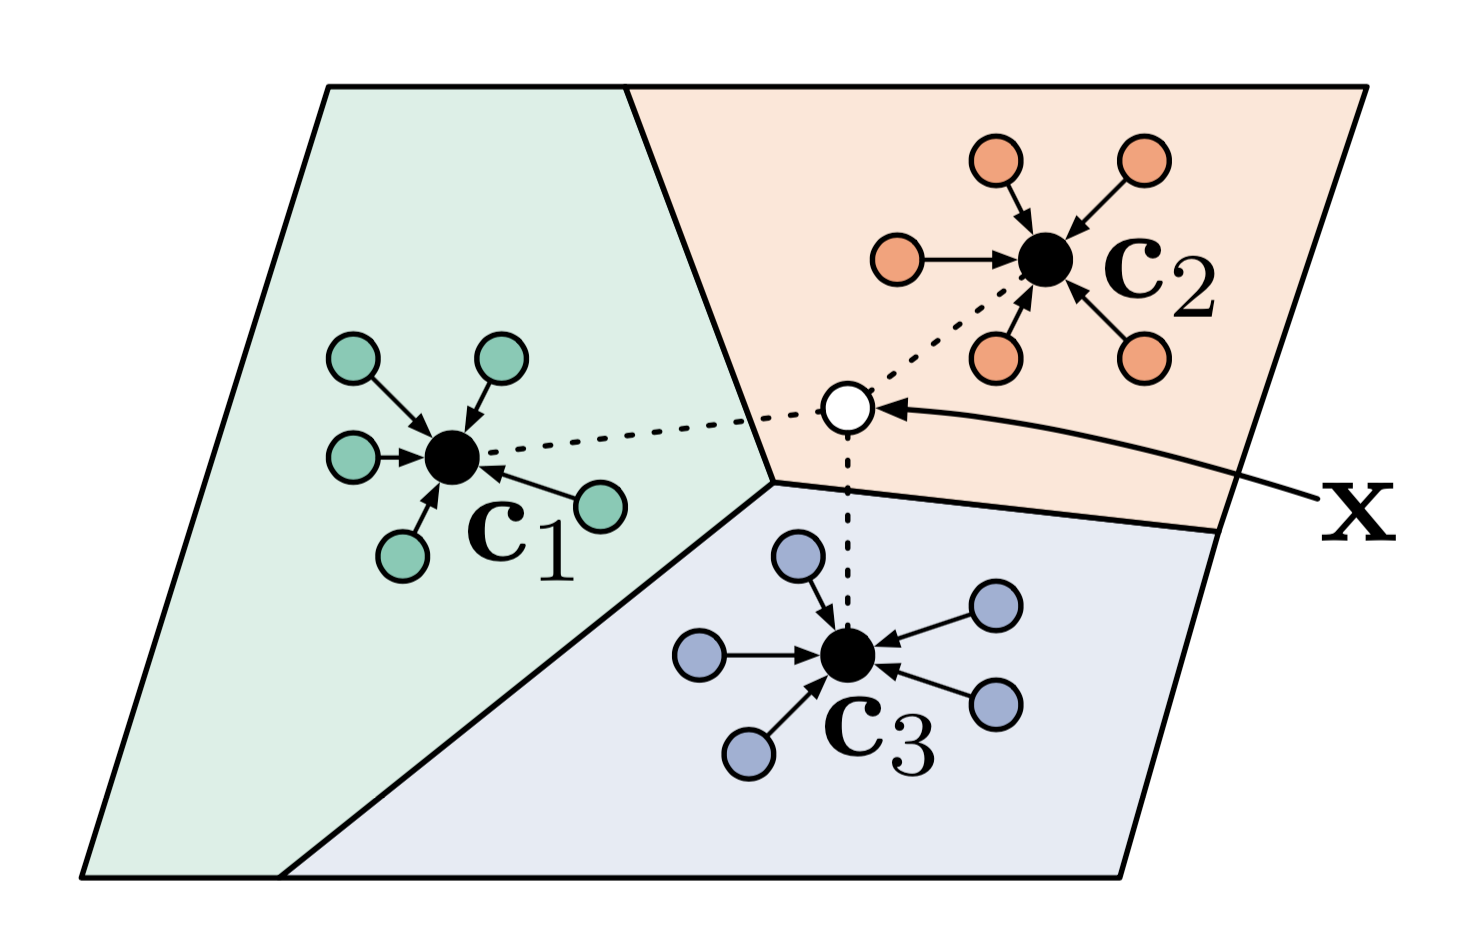
\includegraphics[width=10cm]{figures/prototype}
\caption{Few-shot learning procedure for Prototypical Networks.}\label{fig:proto}
\end{figure}

Prototypical Networks compute an $M$-dimensional representation $c_k\in\mathbb{R}^M$, or \textit{prototype}, of each class through an embedding function $f_{\phi}:\mathbb{R}^D\to\mathbb{R}^M$ with learnable parameters $\phi$. Each prototype is the mean vector of the embedded support points belonging to its class:
\begin{equation}\label{eq:prototype}
c_k=\frac{1}{|S_k|}\sum_{(x_i,y_i)\in S_k}f_{\phi}(x_i)
\end{equation}
Given a distance function $d:\mathbb{R}^M\times\mathbb{R}^M\to[0,+\infty)$, Prototypical Networks produce a distribution over classes for a query point $x$ bases on a softmax over distances to the prototypes in the embedding space
\begin{equation}\label{eq:prediction}
p_{\phi}(y=k|x)=\frac{\exp(-d(f_{\phi}(x),c_k))}{\sum_{k'}\exp(-d(f_{\phi}(x),c_{k'}))}
\end{equation}
Learning proceeds by minimizing the negative log-probability $J(\phi)=-log p_{\phi}(y=k|x)$ of the true class $k$ via SGD. Training episodes are formed by randomly selecting a subset of classes from the training set, then choosing a subset of examples within each class to act as the support set and a subset of the reminder to serve as query points.



\begin{algorithm}
\begin{algorithmic}
\State \textbf{Input} $\mathcal{D}=\{(x_1,y_1),\dots,(x_N,y_N) \}$, where each $y_i\in\{1,\dots,K\}$. $\mathcal{D}_k$ denotes the subsets of $D$ containing all elements $(x_i,y_i)$ such that $y_i=k$.
\State \textbf{Output} The loss $J$ for a randomly generated training episodes.
\State $V\gets \textsc{RandomSample}(\{1,\dots,K\},N_C)$ \Comment{Select class indices for episode}
\For{$k$ in $\{1,\dots,N_C\}$}
    \State $S_k\gets\textsc{RandomSample}(\mathcal{D}_{V_k},N_S)$ \Comment{Select support examples}
    \State $Q_k\gets\textsc{RadnomSample}(\mathcal{D}_{V_k\setminus S_k},N_Q)$ \Comment{Select query examples}
    \State $c_k\gets\frac{1}{N_C}\sum_{(x_i,y_i)\in S_k} f_{\phi}(x_i)$ \Comment{Compute prototype from support examples}
\EndFor
\State $J\gets 0$ \Comment{Initialize loss}
\For{$k$ in $\{1,\dots,N_C \}$}
\For{$(x,y)$ in $Q_k$}
\State $J\gets J+\frac{1}{N_C N_Q}\left[d(f_{\phi}(x),c_k)+\log\sum_{k'}\exp(-d(f_{\phi}(x),c_{k'})) \right]$ \Comment{Update loss}
\EndFor
\EndFor
\end{algorithmic}
\caption{Training episode loss computation for Prototypical Networks.}
\end{algorithm}

\paragraph{Prototypical Networks as Mixture Density Estimation} For a particular class of distance functions, Bregman divergences \cite{banerjee2005clustering}, the Prototypical Networks is equivalent to performing mixture density estimation on the support set with an exponential family density. Examples of Bregman divergences include squared Euclidean distance $\|z-z'\|_2^2$.

Prototype computation can be viewed in terms of hard clustering on the support set, with one cluster per class and each support point assigned to its corresponding class cluster. It has been shown for Bregman divergences that the cluster representative achieving minimal distance to its assigned points is the cluster mean. Thus the prototype computation in Equation (\ref{eq:prototype}) yields optimal cluster representatives given the support set labels when a Bregman divergence is used.

Moreover, any regular exponential family distribution $p_{\psi}(z|\theta)$ with parameters $\theta$ and cumulant function $\psi$ can be written in terms of a uniquely determined regular Bregman divergence
\begin{equation}
p_{\psi}(z|\theta)=\exp(z^T\theta-\psi(\theta)-g_{\psi}(z))=\exp(-d_\varphi(z,\mu(\theta))-g_{\varphi}(z))
\end{equation}
Consider now a regular exponential family mixture model with parameters $\Gamma=\{\theta_k,\pi_k\}_{k=1}^K$
\begin{equation}
p(z|\Gamma)=\sum_{k=1}^K\pi_k p_{\psi}(z|\theta_k)=\sum_{k=1}^K\exp(-d_{\varphi}(z,\mu(\theta_k))-g_{\varphi}(z))
\end{equation}
Given $\Gamma$, inference of the cluster assignment $y$ for an unlabeled point $z$ becomes
\begin{equation}\label{eq:inference}
p(y=k|z)=\frac{\pi_k\exp(-d_{\varphi}(z,\mu(\theta_k)))}{\sum_{k'}\pi_{k'}\exp(-d_{\varphi}(z,\mu(\theta_k)))}
\end{equation}
For an equally-weighted mixture model with one cluster per class, cluster assignment inference (\ref{eq:inference}) is equivalent to query class prediction (\ref{eq:prediction}) with $f_{\phi}(x)=z$ and $c_k=\mu(\theta_k)$. In this case, Prototypical Networks are effectively performing mixture density estimation with an exponential family distribution determined by $d_{\varphi}$. The choice of distance therefore specifies modeling assumptions about the class-conditional data distribution in the embedding space.

\subsection{Meta Learning}

\cite{ravi2016optimization} introduced a meta-learning method where an LSTM updates the weights of a classifier for a given episode. \cite{munkhdalai2017meta} also presented a meta-learning architecture that learns meta-level knowledge across tasks, and it changes its inductive bias via fast parameterization. \cite{finn2017model} is using a model agnostic meta-learner based on gradient descent, the goal is to train a classification model such that given a new task, a small amount of gradient steps with few data will be enough to generalize. \cite{mishra2017meta} used Temporal Convolutions which are deep recurrent networks based on dilated convolutions, this method also exploits contextual information from the subset $\mathcal{T}$ providing very good results.

\subsection*{Meta-Learner}

In this part, I will use meta-learner \cite{ravi2016optimization} to illustrate the idea of meta learning.

Consider a single dataset, or episode, $D$ which includes $D_{\text{train}}$ and $D_{\text{test}}$. Suppose we have a learner neural net classifier with parameter $\theta$ that we want to train on $D_{\text{train}}$. The standard optimization problems used to train deep neural networks are some variant of gradient descent, which uses updates of the form
\begin{equation}
\theta_t=\theta_{t-1}-\alpha_t\nabla_{\theta_{t-1}}\mathcal{L}_t
\end{equation}
where $\theta_{t-1}$ are the parameters of the learner after $t-1$ updates, $\alpha_t$ is the learning rate at time $t$, $\mathcal{L}_t$ is the loss optimized by the learner for its $t^{\text{th}}$ update, $\nabla_{\theta_{t-1}}\mathcal{L}_t$ is the gradient of the loss with respect to parameters $\theta_{t-1}$, and $\theta_t$ is the updated parameters of the learner. 

The key observation that the meta learner model leverage is that this update resembles the update for the cell state in LSTM
\begin{equation}
c_t=f_t\odot c_{t-1}+i_t\odot\tilde{c}_t
\end{equation}
if $f_t=1,c_{t-1}=\theta_{t-1},i_t=\alpha_t$, and $\tilde{c}_t=-\nabla_{\theta_{t-1}}\mathcal{L}_t$.

Thus the authos propose training a meta-learner LSTM to \textbf{learn an update rule} for training a neural network. The cell state of the LSTM to be the parameters of the learner, or $c_t=\theta_t$, and the candidate cell state $\tilde{c}_t=\nabla_{\theta_{t-1}}\mathcal{L}_t$, given how valuable information about the gradient is for optimization. Parametric forms for $i_t$ and $f_t$ is defined so that the meta learner can determine optimal values through the course of the updates.

The $i_t$ corresponds to the learning rate for the updates. Let
\[
i_t=\sigma(\mathbf{W}_I\cdot\left[\nabla_{\theta_{t-1}}\mathcal{L}_t,\mathcal{L}_t,\theta_{t-1},i_{t-1} \right]+{\bf b}_I)
\]
meaning that the learning rate is a function of the current parameter value $\theta_{t-1}$, the current gradient $\nabla_{\theta_{t-1}}\mathcal{L}_t$, the current loss $\mathcal{L}_t$, and the previous learning rate $i_{t-1}$. With this information, the meta-learner should be able to \textbf{finely control the learning rate} so as to train the learner quickly while avoiding divergence.

As for $f_t$, it seems possible that the optimal choice isn’t the constant 1. Intuitively, what would justify shrinking the parameters of the learner and forgetting part of its previous value would be if the learner is currently in a bad local optima and needs a large change to escape. This would correspond to a situation where the loss is high but the gradient is close to zero. Thus, one proposal for the forget gate is to have it be a function of that information, as well as the previous value of the forget gate:
\[
f_t=\sigma(\mathbf{W}_F\cdot\left[\nabla_{\theta_{t-1}}\mathcal{L}_t,\mathcal{L}_t,\theta_{t-1},i_{t-1} \right]+{\bf b}_F)
\]

Additionally, notice that we can also learn the initial value of the cell state c0 for the LSTM, treating it as a parameter of the meta-learner. This corresponds to the initial weights of the classifier (that the meta-learner is training). \textbf{Learning this initial value} lets the meta-learner determine the optimal initial weights of the learner so that training begins from a beneficial starting point that allows optimization to proceed rapidly.



% \paragraph{The relationship between data augmentation, few-shot learning, transfer learning} When we face the insufficiency of data 

% \paragraph{Transfer Learning} is a research problem in machine learning that focuses on storing knowledge gained while solving one problem and applying it to a different but related problem. Research on transfer learning has attracted more and more attention since 1995 in different names: \textbf{learning to learn}, life-long learning, knowledge transfer, inductive transfer, multitask learning, knowledge consolidation, context-sensitive learning, knowledge-based inductive bias, \textbf{metalearning}, and incremental/cumulative learning \cite{pan2010survey}.


% \section{Transfer Learning} 

% \begin{definition}[Transfer Learning]
% Given a source domain $\mathcal{D}_S$ and learning task $\mathcal{T}_S$, a target domain $\mathcal{D}_T$ and learning task $\mathcal{T}_T$, transfer learning aims to help improve the learning of target predictive function $f_T(\cdot)$ in $\mathcal{D}_T$ using the knowledge in $\mathcal{D}_S$ and $\mathcal{T}_S$, where $\mathcal{D}_S\neq \mathcal{D}_T$, or $\mathcal{T}_S\neq \mathcal{T}_T$
% \end{definition}

% Based on the definition of transfer learning, we can categorize transfer learning under three subsettings, based on different situations between the source and target domains and tasks \cite{pan2010survey}
% \begin{itemize}
% \item Inductive transfer learning. In the inductive transfer learning setting, the target task is different from the source task, no matter when the source and target domains are the same or not.
% \item Transductive transfer learning. In the transductive transfer learning setting, the source and target tasks are the same, while the source and target domains are different.
% \item Unsupervised transfer learning. In the unsupervised transfer learning setting, the target task is different from but related to the source task. There are no labeled data available in both source and target domains in training.
% \end{itemize}


% Specifically, for neural networks, transfer learning is a technique in which we take pre-trained weights of neural net trained on some similar or more comprehensive data and fine tune certain parameters to best solve a more specific problem.

% \section{Few-shot Learning}

% \section{Generative Adversarial Networks}


% \section{memo}

% \subsection*{DATA AUGMENTATION GENERATIVE ADVERSARIAL NETWORKS}

% traditional transformations not affect the class, not only for low-data cases, train a GAN in source domain, apply it in the low-data domain / target domain, DAGAN does not depend on the classes themselves, data augmentation from a single novel data point?

% dataset, source domain, validation domain, target domain (test domain)



% \subsection*{Matching Networks for One Shot Learning} 



\bibliographystyle{acm}
\bibliography{../references}

\end{document}
